\chapter{两阶段乳腺钼靶分类检测模型weakFaster R-CNN}\label{chap:stage2}

在目标检测领域,主流方法以R-CNN系列为代表的两阶段(生成候选框和预测)以及和YOLO\cite{36Redmon2015You},SSD\cite{37Liu2016SSD}为代表的单阶段。

相比单阶段,两阶段检测模型通常含有一个串行的头部结构,即完成前背景分类和回归后,把中间结果作为Fast RCNN头部的输入再进行一次多分类和位置回归。这种设计带来了一些优点:

\begin{itemize}
    \item 对检测任务的解构,先进行前背景的分类,再进行物体的分类,这种解构使得监督信息在不同阶段对网络参数的学习进行指导。
    \item RPN网络为Fast RCNN网络提供良好的先验,并有机会整理样本的比例,减轻Fast RCNN网络的学习负担。
\end{itemize}

虽然两阶段模型存在空间负担大,时间复杂度高等问题,但对于医生而言,更关注的是准确率以及可解释性,所以本文考虑采用更加成熟稳定的Faster RCNN模型。Faster RCNN分为Region Proposal Network(RPN)和Fast R-CNN网络,具体可以分为将特征抽取(Feature Extractor),Proposal提取,ROI Pooling,bounding box regression,classification几个部分。RPN主要负责提取候选框,经过proposal提取产生了大量的候选框(Proposal),选择出包含物体的anchors,映射到共享的特征图上,之后将这些proposal经过ROI Pooling生成统一大小的特征图,再进行后续的Fast R-CNN更进一步的精调。所以Faster R-CNN能否训练成功的关键在于所提取的特征图是否拥有足够的信息,以及RPN能够准确选择出候选框,以及最后的Fast R-CNN网络训练的是否能够拥有区分不同类别的能力。

传统的自然图像尺寸一般为500×500像素,所要识别的目标占据图片主体,且目标之间在大小,形态等各维度均存在较大的差别。在该项目中,由于肿块占比很小,而且negative也常常拥有一些与positive中恶性肿块相似的区域,给准确检测带来了很大的困难。


\section{目的}
根据乳腺钼靶上的定义,对于肿块这种病灶类型,positive和negative之间的区别只存在于边缘的区别。对于传统的Faster R-CNN,如果能够拥有正常样本中疑似恶性图片的病灶标注,那么这个问题并不太难,相当于让模型进行三分类(positive+negative+背景)检测问题,但问题在于本文并没有标注的negative数据。考虑到存在没有标注的信息,而且positive及negative之间的区别非常微小,所以初步设想是希望能够引入弱监督学习的方式,基于原始的Faster R-CNN模型,训练学习positive中恶性病灶信息,进而得到negative中疑似恶性病灶的标注框,而这也是两阶段乳腺钼靶分类检测算法模型weakFaster R-CNN提出的初衷,希望使用两次Faster R-CNN,第一阶段获取negative中疑似恶性病灶的标注框,相当于通过模型人为地给negative赋予标签,这可以为之后第二阶段的进一步使用Faster R-CNN模型检测学习positive及negative之间的微弱区别提供帮助。

第一阶段本文先用使用positive图片数据训练模型,得到一个可以自动检测恶性肿块的网络,当然由于只训练含有恶性肿块的图片,该网络不可避免也会将许多与之相似的良性肿块判断为恶性肿块。

第二阶段,本文用这个模型训练去预测negative图片数据,得到相应的疑似肿块区域,由于已知这些区域非恶性肿块,本文将此归为单独的一类,将此类标注框与原有的恶性标注框共同训练,得到一个具有二分类目标检测的网络,最后将第二阶段得到的模型去预测所有的图片,得到最终的结果。

\section{模型图}
\begin{figure}[!htbp]
    \centering
    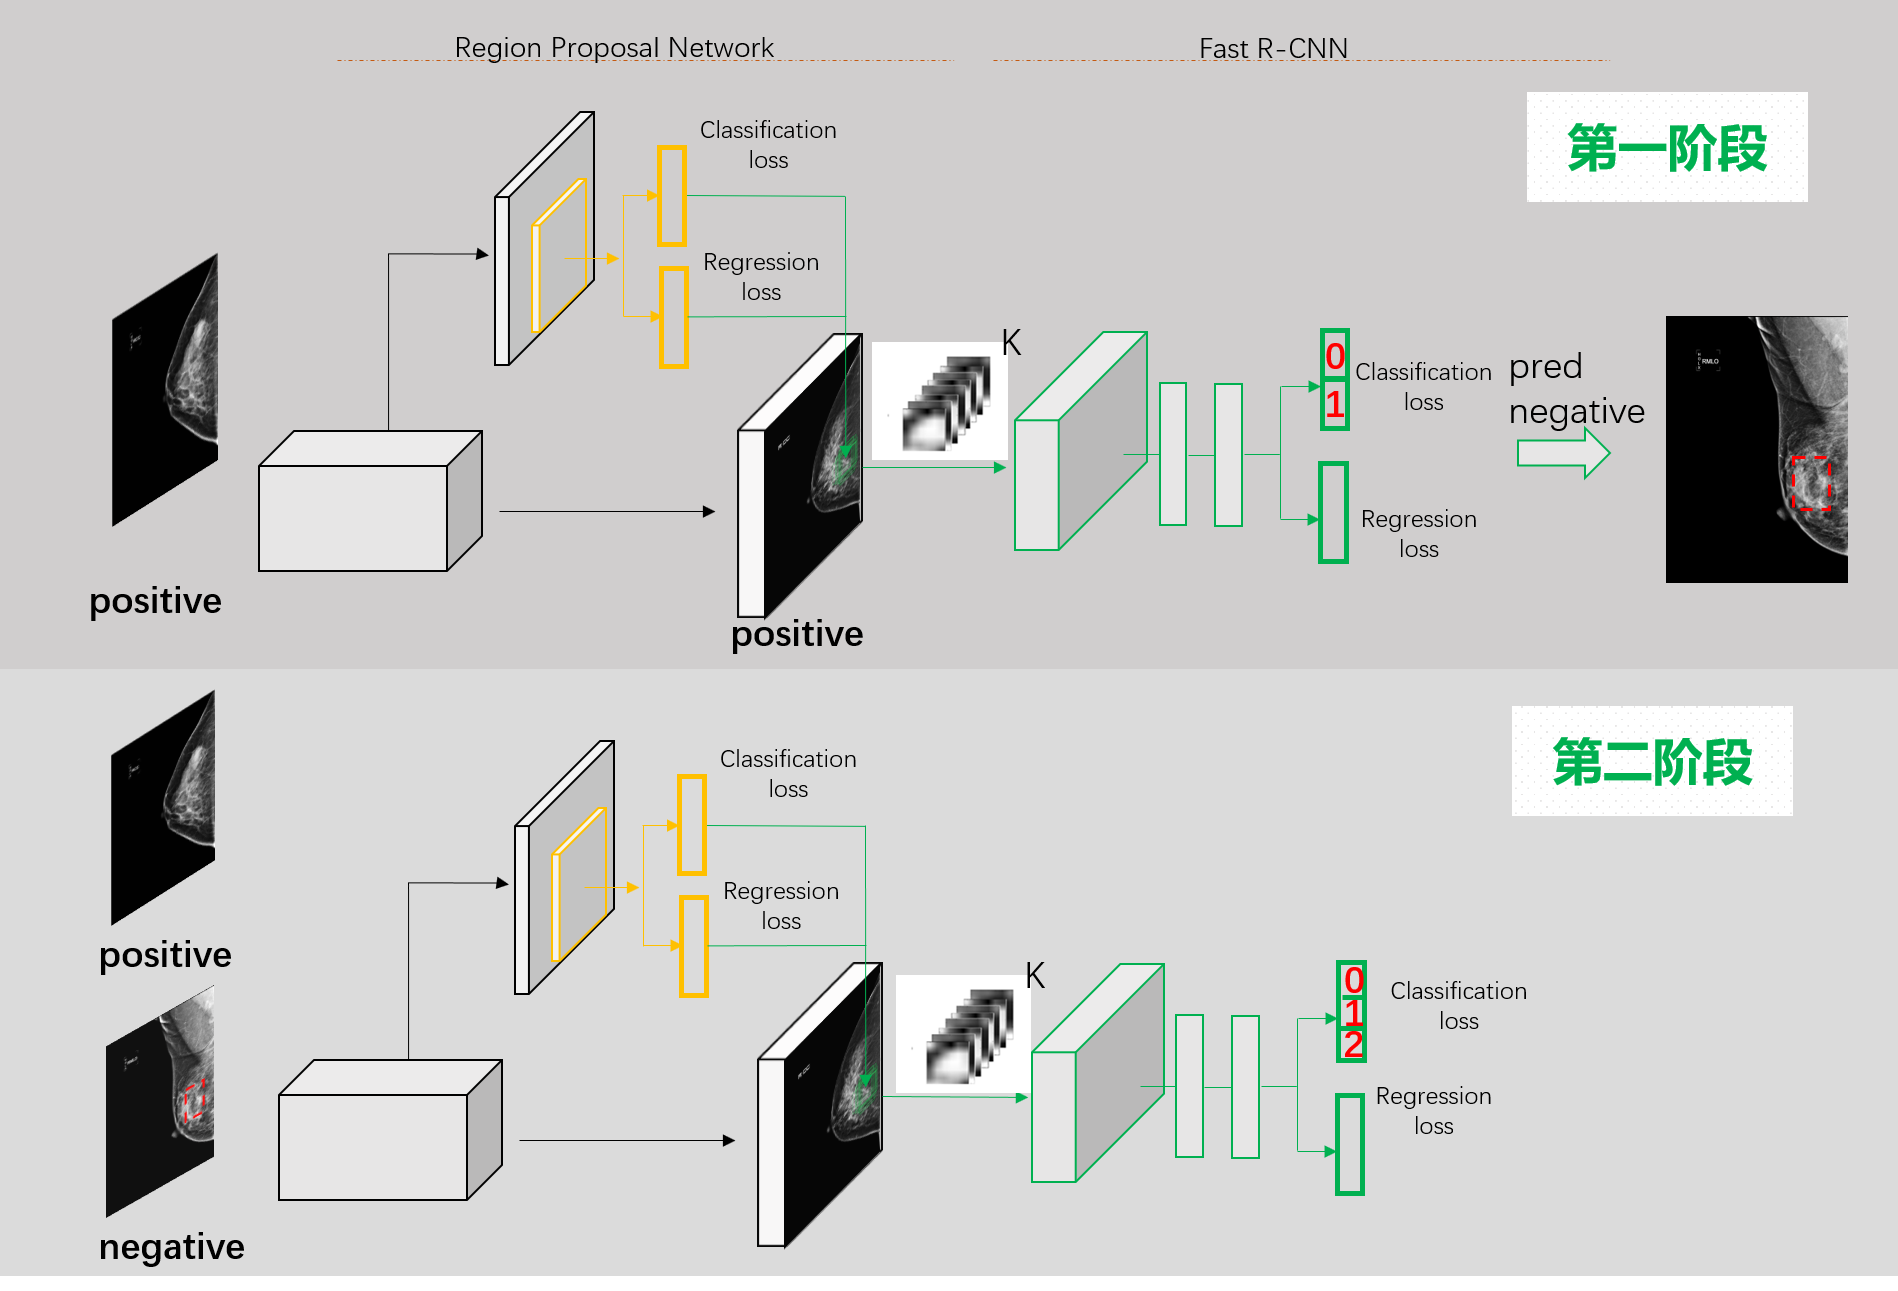
\includegraphics[width=1.0\textwidth]{stage2_model}
    \bicaption{weakFaster R-CNN模型图}{Architecture of weakFaster R-CNN}
    \label{fig:stage2_model}
\end{figure}
weakFaster R-CNN(模型图如图\ref{fig:stage2_model})由于分别使用Faster R-CNN进行两次训练,所以存在两个不同的Faster R-CNN模型,这两个Faster R-CNN的结构和参数量和原始的Faster R-CNN相同。所不同的在于对数据的输入以及数据后处理方面。在数据输入方面,第一阶段只有positive图片,第二阶段则包含postive和被第一阶段模型预测出包含有高度疑似恶性病灶的negative图片数据;数据后处理时,在第一阶段应该将训练好的模型去预测negative图片,从而能够与positive图片进行融合,继续第二阶段的训练。如图\ref{fig:stage2_model}所示,第一阶段预测出的negative中病灶位置确实疑似恶性。
\begin{itemize}
    \item 主干网络 
    
    深度残差网络(Deep residual network,ResNet\cite{8he2016deep})的提出是CNN图像史上的一件里程碑事件,在ILSVRC取得了五项第一。从经验来看,网络的深度能够有效提取出模型的高层信息,从而增强模型的学习能力。然而,随着模型层数的加深,以往的模型存在网络深度增加时,网络准确度出现饱和,甚至出现下降的问题。Resnet通过残差学习(如图\ref{fig:stage2_resblock})来解决退化问题,有效解决了深度所造成的模型无法收敛的问题,这称得上是深度网络的一个历史大突破。本文采取Resnet101作为Faster R-CNN的主干网络,借此强大的模型可以充分提取出分类和检测所需要的特征表达,从而提升模型的整体性能。其网络配置如表\ref{tab:stage2_resmodel}。

\begin{figure}[!htbp]
    \centering
    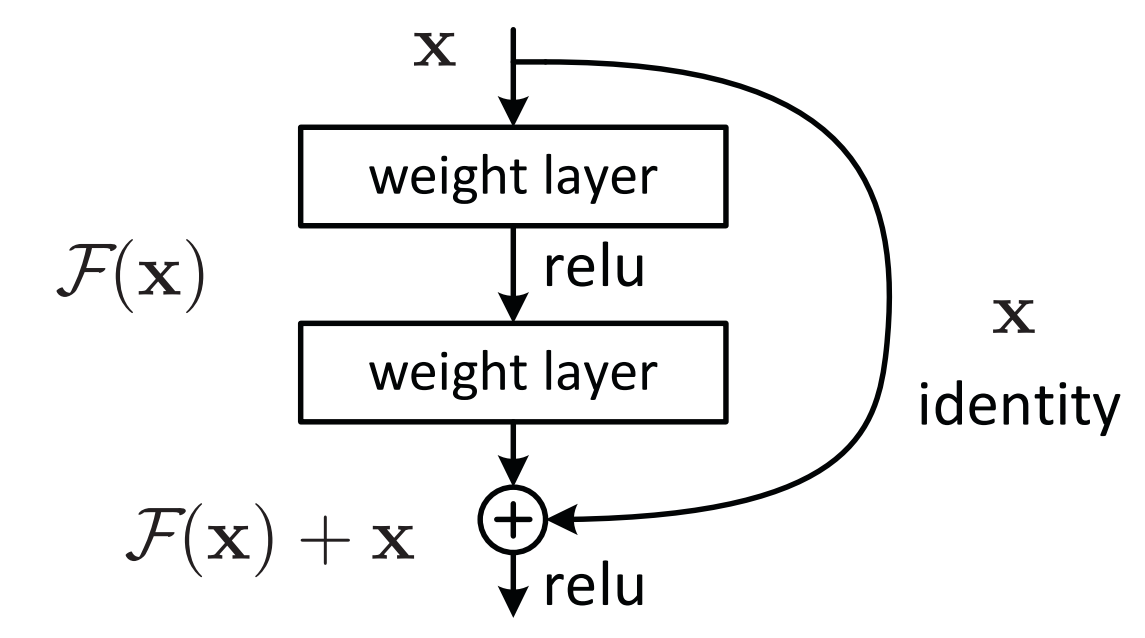
\includegraphics[width=0.7\textwidth]{stage2_resblock}
    \bicaption{残差模块\cite{8he2016deep}}{residual block\cite{8he2016deep}}
    \label{fig:stage2_resblock}
\end{figure}

%\newcommand{\tabincell}[2]{\begin{tabular}{@{}#1@{}}#2\end{tabular}}
\begin{table}[!htbp]
    \bicaption{Resnet101参数配置\cite{8he2016deep}}{The config of Resnet101\cite{8he2016deep}}
    \label{tab:stage2_resmodel}
    \centering
    \footnotesize% fontsize
    \setlength{\tabcolsep}{4pt}% column separation
    %\renewcommand{\arraystretch}{1.2}%row space 
    \begin{tabular}{c|c|c|c|c}
        \hline
        
         layer name& output size &\multicolumn{3}{c}{101-layer} \\
        \hline
         conv1 & 112$\times$112 & \multicolumn{3}{c}{7$\times$7, 64, stride 2}\\
         \hline
         conv2\_x & 56$\times$56 & \multicolumn{3}{c}{3$\times$3 max pool, stride 2} \\
         \hline
         conv2\_x & 56$\times$56 & \multicolumn{3}{c}{$\left[ \begin{array}{c}{1 \times 1,64} \\ {3 \times 3,64} \\ {1 \times 1,256}\end{array}\right] \times 3$}\\    
         \hline
        conv3\_x & 28$\times$28 & \multicolumn{3}{c}{$\left[ \begin{array}{c}{1 \times 1,128} \\ {3 \times 3,128} \\ {1 \times 1,512}\end{array}\right] \times 4$}\\
        \hline
        conv4\_x & 14$\times$14 & \multicolumn{3}{c}{$\left[ \begin{array}{c}{1 \times 1,256} \\ {3 \times 3,256} \\ {1 \times 1,1024}\end{array}\right] \times 23$}\\
        \hline
        conv5\_x & 7$\times$7 & \multicolumn{3}{c}{$\left[ \begin{array}{c}{1 \times 1,512} \\ {3 \times 3,512} \\ {1 \times 1,2048}\end{array}\right] \times 3$}\\
        \hline
        & 1$\times$1 &\multicolumn{3}{c}{average pool, 1000-d fc, softmax} \\
        \hline
    \end{tabular}
\end{table}

\begin{comment}
%\newcommand{\tabincell}[2]{\begin{tabular}{@{}#1@{}}#2\end{tabular}}
\begin{table}[!htbp]
    \bicaption{Resnet101参数配置\cite{8he2016deep}}{The config of Resnet101\cite{8he2016deep}}
    \label{tab:stage2_resmodel}
    \centering
    \footnotesize% fontsize
    \setlength{\tabcolsep}{4pt}% column separation
    %\renewcommand{\arraystretch}{1.2}%row space 
    \begin{tabular}{c|c|c|c|c}
        \hline
        
         layer name& output size &\multicolumn{3}{c}{101-layer} \\
        \hline
         conv1 & 112$\times$112 & \multicolumn{3}{c}{7$\times$7, 64, stride 2}\\
         \hline
         \multirow{2}{*}{conv2\_x} & \multirow{2}{*}{56$\times$56} & \multicolumn{3}{c}{3$\times$3 max pool, stride 2} \\
		\cline{3-5}         
         & &\multicolumn{3}{c}{$\left[ \begin{array}{c}{1 \times 1,64} \\ {3 \times 3,64} \\ {1 \times 1,256}\end{array}\right] \times 3$}\\
         \hline
        conv3\_x & 28$\times$28 & \multicolumn{3}{c}{$\left[ \begin{array}{c}{1 \times 1,128} \\ {3 \times 3,128} \\ {1 \times 1,512}\end{array}\right] \times 4$}\\
        \hline
        conv4\_x & 14$\times$14 & \multicolumn{3}{c}{$\left[ \begin{array}{c}{1 \times 1,256} \\ {3 \times 3,256} \\ {1 \times 1,1024}\end{array}\right] \times 23$}\\
        \hline
        conv5\_x & 7$\times$7 & \multicolumn{3}{c}{$\left[ \begin{array}{c}{1 \times 1,512} \\ {3 \times 3,512} \\ {1 \times 1,2048}\end{array}\right] \times 3$}\\
        \hline
        & 1$\times$1 &\multicolumn{3}{c}{average pool, 1000-d fc, softmax} \\
        \hline
    \end{tabular}
\end{table}
\end{comment}

\begin{comment}
\begin{table}[!htbp]
    \bicaption{Resnet101参数配置}{The config of Resnet101}
    \label{tab:stage2_resmodel}
    \centering
    \footnotesize% fontsize
    \setlength{\tabcolsep}{4pt}% column separation
    %\renewcommand{\arraystretch}{1.2}%row space 
    \begin{tabular}{c|c|c|c|c}
        \hline
        
         layer name& output size &\multicolumn{3}{c}{101-layer} \\
        \hline
         conv1 & 112$\times$112 & \multicolumn{3}{c}{7$\times$7, 64, stride 2}\\
        \hline
        conv2\_x& 56$\times$56 & \multicolumn{3}{c}{$\left[ \begin{array}{c}{1 \times 1,64} \\ {3 \times 3,64} \\ {1 \times 1,256}\end{array}\right] \times 3$}\\
        \hline
        conv3\_x & 28$\times$28 & \multicolumn{3}{c}{$\left[ \begin{array}{c}{1 \times 1,128} \\ {3 \times 3,128} \\ {1 \times 1,512}\end{array}\right] \times 4$}\\
        \hline
        conv4\_x & 14$\times$14 & \multicolumn{3}{c}{$\left[ \begin{array}{c}{1 \times 1,256} \\ {3 \times 3,256} \\ {1 \times 1,1024}\end{array}\right] \times 23$}\\
        \hline
        conv5\_x & 7$\times$7 & \multicolumn{3}{c}{$\left[ \begin{array}{c}{1 \times 1,512} \\ {3 \times 3,512} \\ {1 \times 1,2048}\end{array}\right] \times 3$}\\
        \hline
        & 1$\times$1 &\multicolumn{3}{c}{average pool, 1000-d fc, softmax} \\
        \hline
    \end{tabular}
\end{table}
\end{comment}

在本文中,无论是两阶段还是一阶段模型,本文均采用该模型作为检测模型的主干网络。具体而言,特征提取模块取conv1,conv2,conv3和conv4,之后再使用Fast R-CNN模块取conv5作为高层语义的提取器。
\item ROI Align 

ROI Align 是在Mask R-CNN\cite{62he2017mask}这篇论文里提出的一种区域特征聚集方式, 很好地解决了ROI Pooling操作中两次量化造成的区域不匹配的问题。原始的ROI Pooling过程需要首先根据后面网络要求的输入尺寸求网格大小,如输入特征图尺寸为5×5,而网络输入尺寸为2×2,那么网格按照5/2=2个像素点对网格进行切分;其次对于每个小网格,求最大值作为该网格最大池化之后的值。ROI Pooling过程会有两次量化过程,对于一个Region Proposal,首先从原图经过全卷积网络到特征图,得到的候选框位置可能存在浮点数,进行取整操作从而出现第一次量化;其次,在ROI Pooling求取每个小网格的位置时也同样存在浮点数取整的情况。这两次量化的结果都使得候选框的位置会出现偏差。

为了解决上述缺点,本文使用了ROI Align的方法。思路很简单:取消量化操作,使用双线性内插的方法获得坐标为浮点数的像素点上的图像数值,从而将整个特征聚集过程转化为一个连续的操作。在检测测任务中将 ROI Pooling 替换为 ROI Align 可以提升检测模型的准确性。

\end{itemize}

\section{训练过程与细节}
\subsection{训练步骤}
\begin{itemize}
	\item 按照第二张数据预处理和数据划分的方式对数据进行处理;考虑到训练集中恶性和正常样本比达到1:3,非常悬殊。实际训练过程中对恶性样本进行上下左右四种方式进行数据扩增,对良性数据只进行左右翻转方式。
	\item 按照第一阶段思路,只取出训练集中positive图片及其标注文件,并按照Faster R-CNN输入要求,将训练集数据进行相应操作(包括基本的数据预处理操作);进行模型调参工作,查看损失曲线下降情况,得到第一阶段训练后的模型。
	\item 将上述得到的模型对训练集中的所有negative数据进行预测,得到良性标注框,取出这部分标注框与原有的医生标注的恶性标注框进行合并,得到第二阶段需要的训练数据。
	\item 将上述得到的数据给Faster R-CNN模型再次训练,再次通过具体的调参,查看损失曲线等方式,最终得到第二阶段的模型。至此,在训练集上已经对所有数据都进行训练过了。
	\item 将上述得到的模型对所有的测试集图片数据进行训练,之后按照一定的标准得到对应的病例的评判结果。
\end{itemize}

本文借鉴了迁移学习的思路,对于低层语义采用较小的学习率进行调整,对于高层语义,也就是conv5 block,本文冻结了除最后两个卷积层外的参数。
\subsection{第一阶段}
第一阶段只考虑训练集中478张恶性图片,经过上述数据预处理和扩增方式后,恶性样本总数达到1912(478×4)。主要参数设置如表\ref{tab:2_stage_1_training_config}所示。
\begin{table}[!htbp]
    \bicaption{weakFaster R-CNN第一阶段训练参数配置}{The first stage training parameter configuration of weakFaster R-CNN}
    \label{tab:2_stage_1_training_config}
    \centering
    \footnotesize% fontsize
    \setlength{\tabcolsep}{4pt}% column separation
    \renewcommand{\arraystretch}{1.2}%row space 
    \begin{tabular}{cc}
        \hline
        参数名称& 参数值 \\
        \hline
        Batch\_size & 2 \\
        Learning rate& 1e\_4 \\
        Decay\_steps & 60 \\
        Decay\_rate & 0.1 \\
        Optimizer& adam \\
        \hline
    \end{tabular}
\end{table}
\begin{comment}
打印出训练loss曲线,如图\ref{fig:stage2_trainingloss},
	\begin{figure}[!htbp]
    \centering
    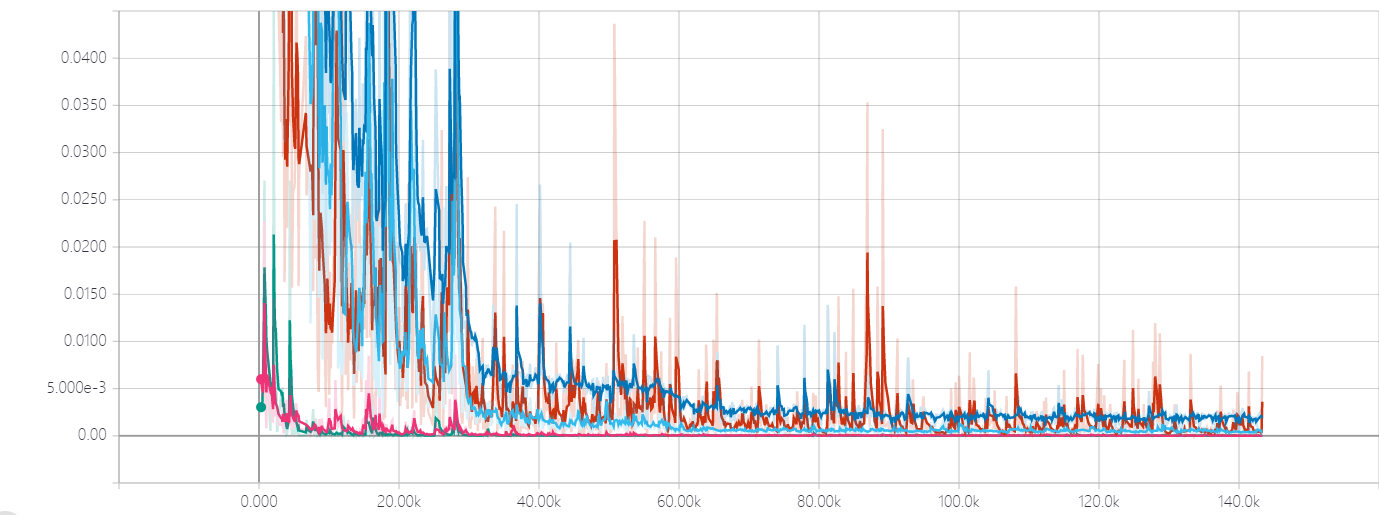
\includegraphics[width=1.0\textwidth]{stage2_trainingloss}
    \bicaption{weakFaster R-CNN第一阶段loss下降曲线}{The first stage loss curve of weakFaster R-CNN}
    \label{fig:stage2_trainingloss}
	\end{figure}
\end{comment}
取损失函数下降足够平稳的140000iters对训练集良阴性(正常样本)进行预测,主要参数设置如表\ref{tab:2_stage_1_pred_config}所示。
\begin{table}[!htbp]
    \bicaption{weakFaster R-CNN第一阶段预测参数配置}{The first stage prediction parameter configuration of weakFaster R-CNN}
    \label{tab:2_stage_1_pred_config}
    \centering
    \footnotesize% fontsize
    \setlength{\tabcolsep}{4pt}% column separation
    \renewcommand{\arraystretch}{1.2}%row space 
    \begin{tabular}{cc}
        \hline
        参数名称& 参数值\\
        \hline
        CONF\_THRESH & 0.8\\
        NMS\_THRESH & 0.3\\
        \hline
    \end{tabular}
\end{table}

结果对训练集中的1858(2336-478)张正常样本,预测出365张有疑似恶性病灶的图片。
对其抽样进行可视化结果如图\ref{fig:stage2_pred_vis}。其中黄框为ground truth,粉红框为预测框。
\begin{figure}[!htbp]
    \centering
    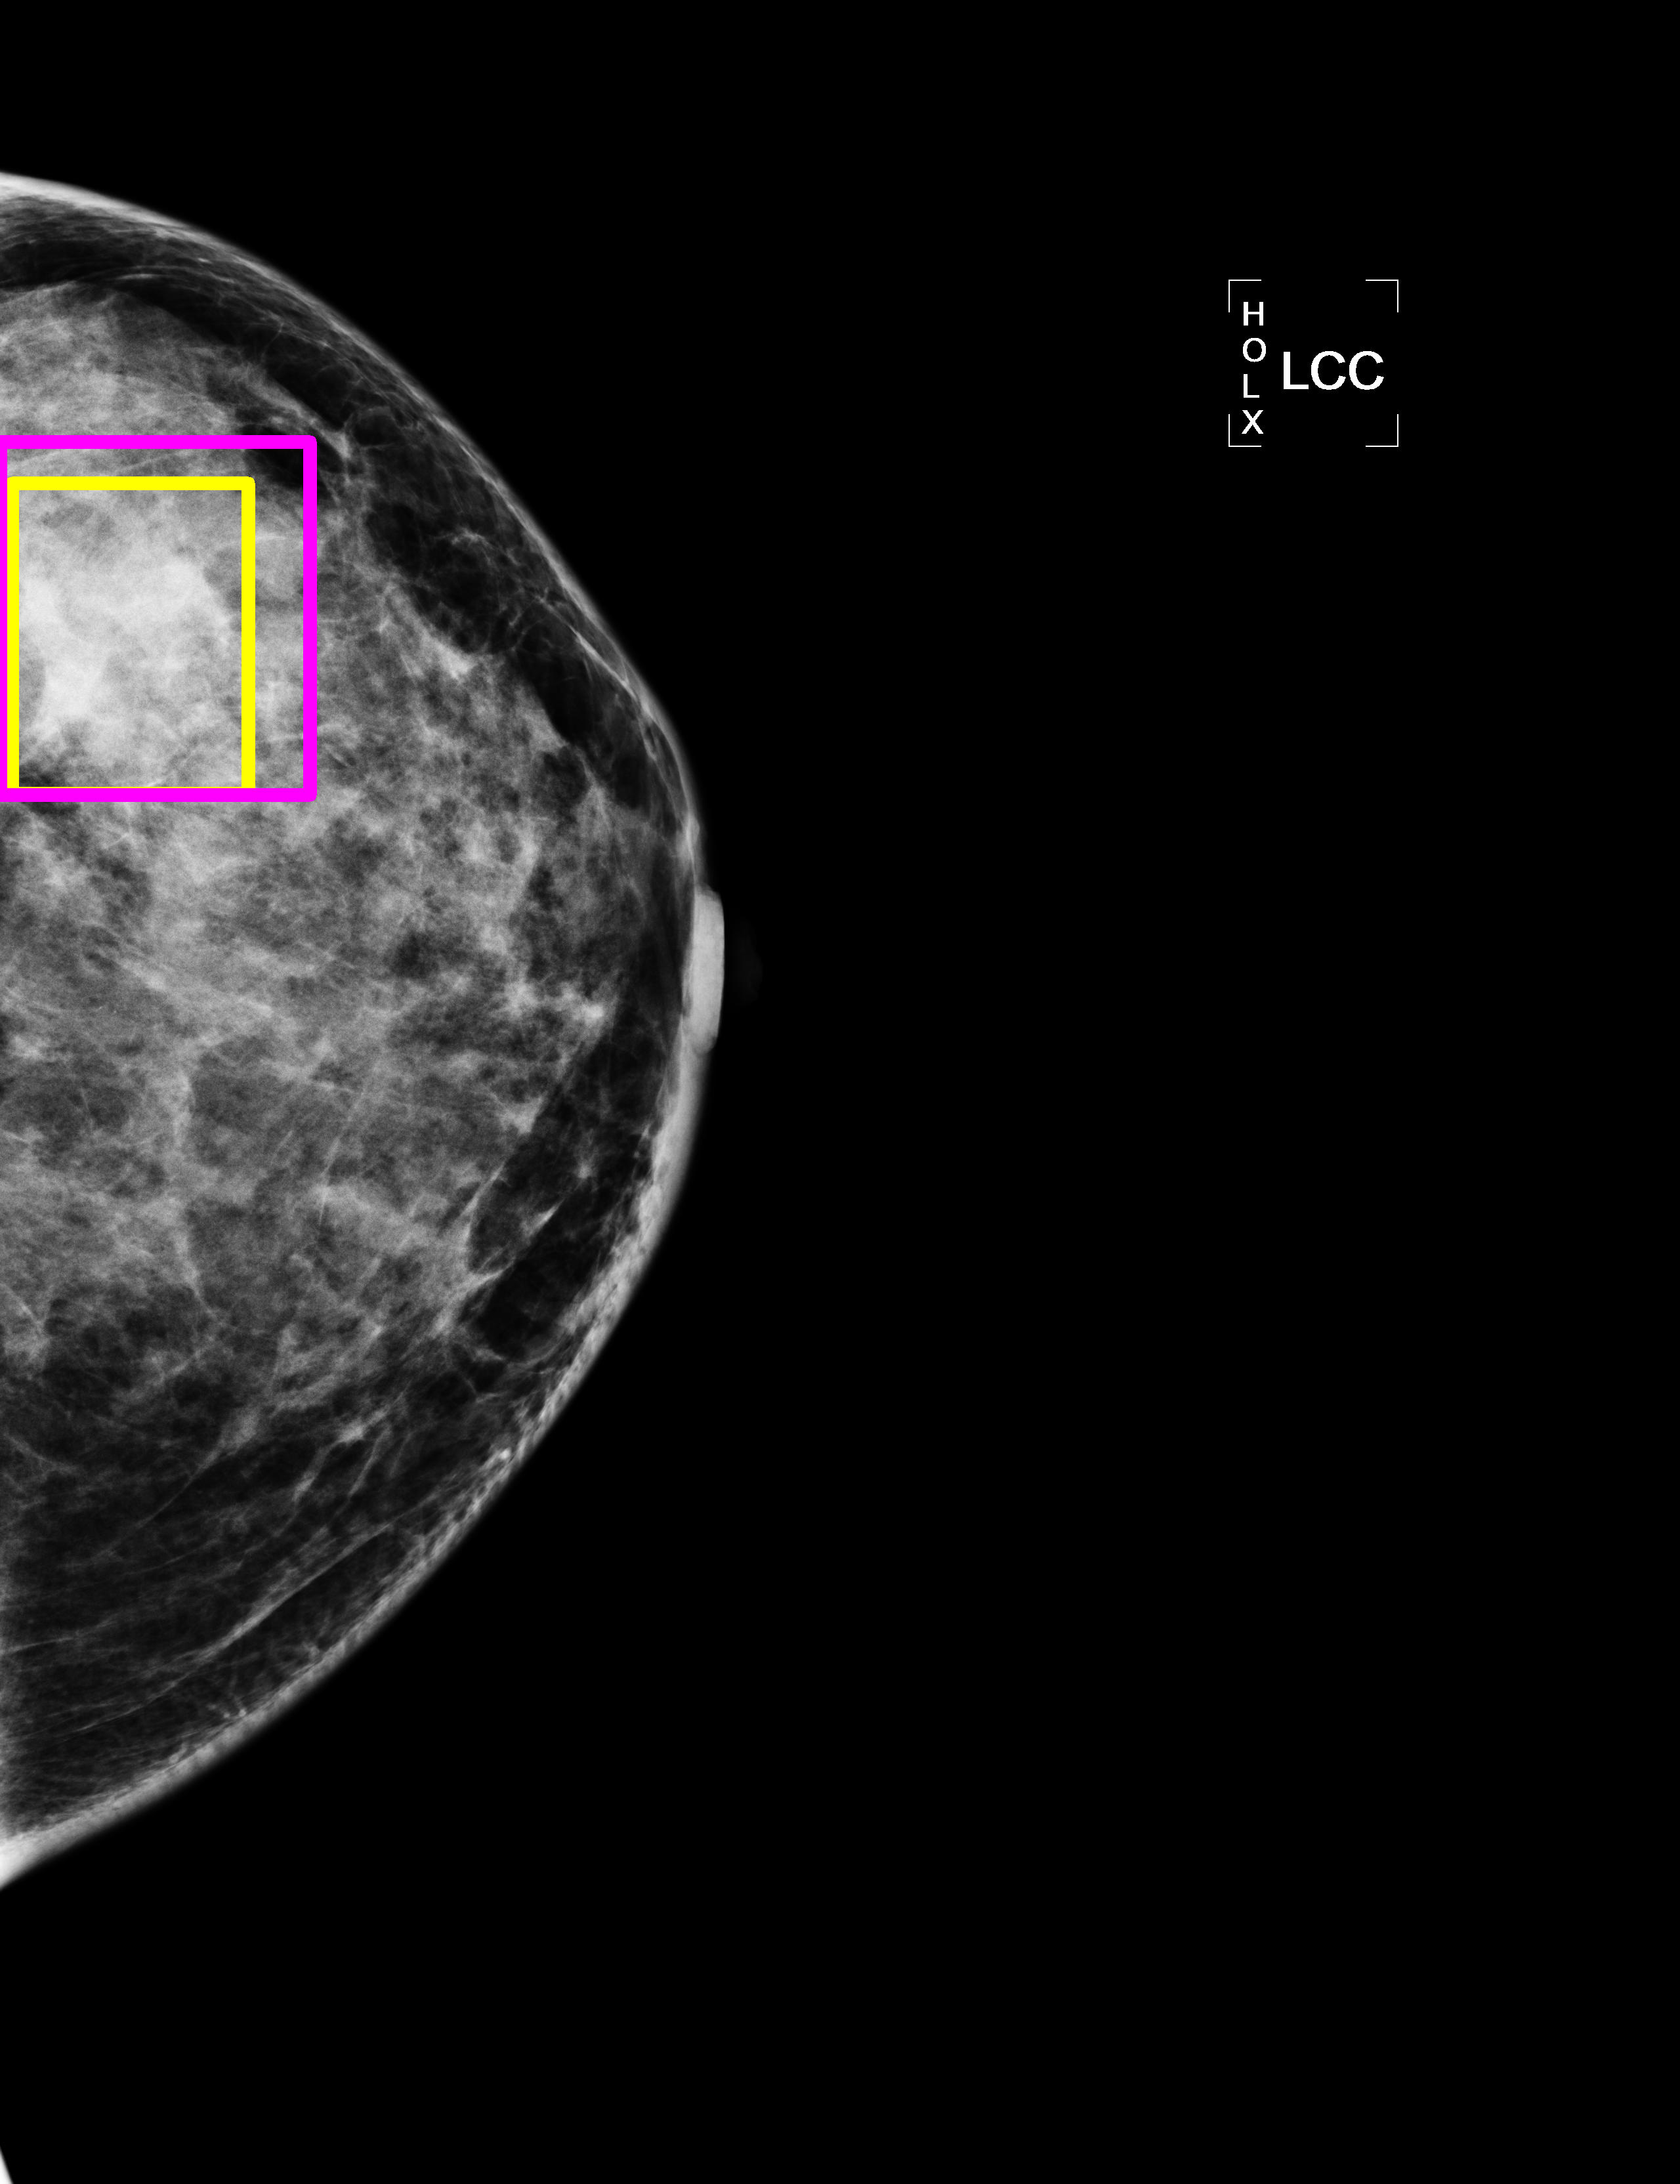
\includegraphics[width=0.40\textwidth]{stage2_pred_vis}
    \bicaption{weakFaster R-CNN第一阶段对图片预测结果可视化}{Visualization of image prediction results in the first stage of a weakFaster R-CNN}
    \label{fig:stage2_pred_vis}
\end{figure}
可以看出,疑似恶性的图片区分得不错。测试集带有恶性标注的恶性图片共120张,预测出102张,对其进行IoU查看,发现预测出来的pred\_bbox与真实的gt的IoU均会大于设置的0.5的阈值,也就是说,120张图片有18张没被正确预测,其他预测正确的均预测正确。

\subsection{第二阶段}
开始进行第二阶段的训练。经过第一阶段,训练集中产生了365张拥有疑似恶性病灶的正常图片样本,合并原有的训练集恶性图片样本468张,是本文第二阶段重点学习的数据。

第二阶段,取原始的恶性病灶图片及第一阶段预测的疑似恶性病灶的正常图片,总共843张(468+365)图片进行训练,经过特定的预处理和数据扩增操作后,开始进行训练。训练过程中,具体参数设置如表\ref{tab:2_stage_2_training_config}所示。
\begin{table}[!htbp]
    \bicaption{weakFaster R-CNN第二阶段训练参数配置}{
The second stage training parameter configuration of weakFaster R-CNN}
    \label{tab:2_stage_2_training_config}
    \centering
    \footnotesize% fontsize
    \setlength{\tabcolsep}{4pt}% column separation
    \renewcommand{\arraystretch}{1.2}%row space 
    \begin{tabular}{cc}
        \hline
        参数名称& 参数值\\
        \hline
        Batch\_size & 2\\
        Learning rate& 1e\_4\\
        Decay\_steps & 60\\
        Decay\_rate & 0.1\\
        Optimizer& adam\\
        \hline
    \end{tabular}
\end{table}

\begin{comment}
下降loss曲线如图\ref{fig:stage2_2_loss}所示。
\begin{figure}[!htbp]
    \centering
    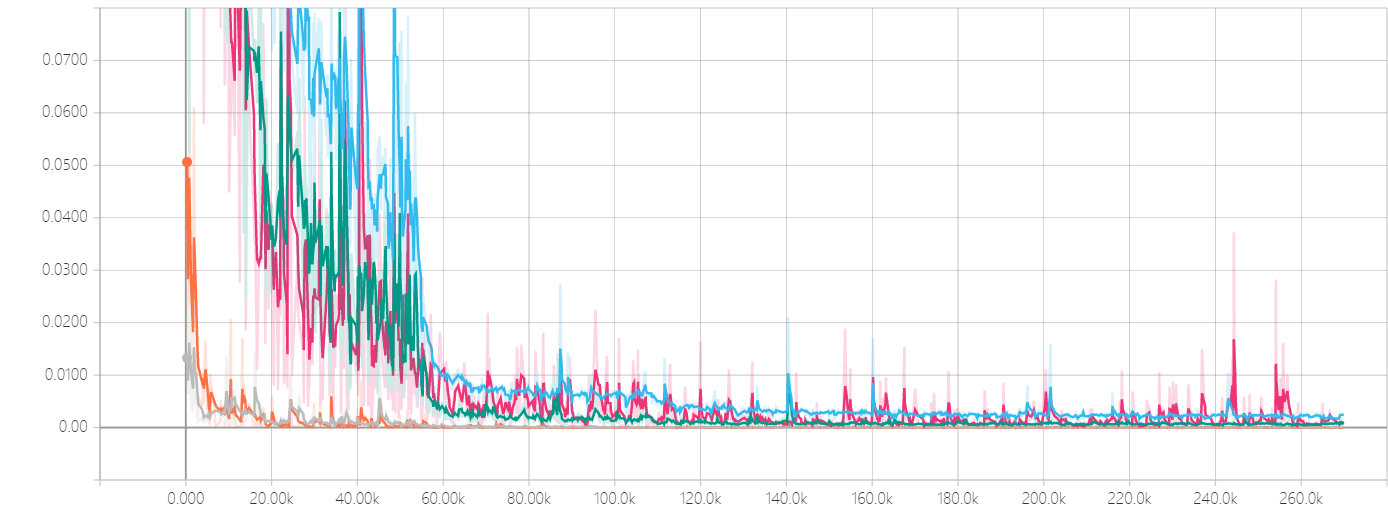
\includegraphics[width=1.0\textwidth]{stage2_2_loss}
    \bicaption{weakFaster R-CNN第二阶段loss下降曲线}{The second stage loss curve of weakFaster R-CNN}
    \label{fig:stage2_2_loss}
\end{figure}
\end{comment}
使用260000iters对训练集进行预测。
训练时的主要参数设置如表\ref{tab:2_stage_2_pred_config}所示。
\begin{table}[!htbp]
    \bicaption{weakFaster R-CNN第二阶段预测参数配置}{
The second stage prediction parameter configuration of weakFaster R-CNN}
    \label{tab:2_stage_2_pred_config}
    \centering
    \footnotesize% fontsize
    \setlength{\tabcolsep}{4pt}% column separation
    \renewcommand{\arraystretch}{1.2}%row space 
    \begin{tabular}{cc}
        \hline
        参数名称& 参数值\\
        \hline
        CONF\_THRESH& 0.7\\
        NMS\_THRESH& 0.4\\
        RPN\_PRE\_NMS\_TOP\_N & 1000\\
        RPN\_POST\_NMS\_TOP\_N & 100\\
        RPN\_NMS\_THRESH & 0.8\\    
        \hline
    \end{tabular}
\end{table}
\section{结果讨论与分析}

训练集共有578个病例,其中恶性病例244个,预测结果如表\ref{tab:2_stage_2_pred_result_in_training_set}所示。
\begin{table}[!htbp]
    \bicaption{weakFaster R-CNN第二阶段训练集预测结果}{
The prediction result for training set in the second stage of weakFaster R-CNN}
    \label{tab:2_stage_2_pred_result_in_training_set}
    \centering
    \footnotesize% fontsize
    \setlength{\tabcolsep}{4pt}% column separation
    \renewcommand{\arraystretch}{1.2}%row space 
    \begin{tabular}{ccc}
        \hline
        &真实为恶性(244例)& 真实为良阴性(334例)\\
        \hline
        预测为恶性& 215 &23 \\
        预测为良阴性& 29 &311 \\
        \hline
    \end{tabular}
\end{table}
共预测578例病人,其中恶性244例,正常334例,真实为恶性且判断为恶性(TP)为215例,真实为恶性且判断为阴良性(FP,假阳性数目)为23例,真实为良阴性且判断为良阴性(TN)为311例,真实为良阴性且判断为恶性的(FN)为29例。

\begin{comment}
此时体现的几个基于病例的指标结果如下:
\begin{itemize}
	\item 召回率88\%
	\item 精确度90\%
	\item 准确率91\%
\end{itemize}

预测结果如表\ref{tab:2_stage_2_pred_result_in_testing_set}所示,其中TP为51例,TN为71例,FP为12例,FN为9例。。
\begin{table}[!htbp]
    \bicaption{weakFaster R-CNN第二阶段测试集预测结果}{
The prediction result of testing set in the second stage of weakFaster R-CNN}
    \label{tab:2_stage_2_pred_result_in_testing_set}
    \centering
    \footnotesize% fontsize
    \setlength{\tabcolsep}{4pt}% column separation
    \renewcommand{\arraystretch}{1.2}%row space 
    \begin{tabular}{ccc}
        \hline
        &真实为恶性(60例)& 真实为良阴性(83例)\\
        \hline
        预测为恶性& 51 &12 \\
        预测为良阴性& 9 &71 \\
        \hline
    \end{tabular}
\end{table}
召回率为85\%,精确度为81\%,准确率为85\%。
\end{comment}
经过在训练集上的查看,可知weakFaster R-CNN训练足够充分,开始考虑模型在测试集上的性能。
\subsection{基于病例}
测试集共有143例病人,其中恶性病例60例,正常病例83例。
运行结果显示如表\ref{tab:2_stage_2_pred_result_based_on_patient}所示,
\begin{table}[!htbp]
    \bicaption{weakFaster R-CNN基于病例预测结果}{
The prediction results of weakFaster R-CNN based on patient}
    \label{tab:2_stage_2_pred_result_based_on_patient}
    \centering
    \footnotesize% fontsize
    \setlength{\tabcolsep}{4pt}% column separation
    \renewcommand{\arraystretch}{1.2}%row space 
    \begin{tabular}{ccccc}
        \hline
        &AUC& ACC &SEN &SPE\\
        \hline
        weakFaster R-CNN& 0.8467 &0.9123 &0.8846 &0.9123  \\
        \hline
    \end{tabular}
\end{table}
从结果上可以看出,weakFaster R-CNN能够在一定程度上有效地区分恶性样本和正常样本,使得预测结果中的召回率(SEN)和特异度(SPE)都较高,能够基本满足医院的实际需求。

\subsection{基于图片}
运行结果显示如图\ref{tab:2_stage_2_pred_result_based_on_image}所示,乳腺钼靶的mAP达到0.40,并经过
\begin{table}[!htbp]
    \bicaption{weakFaster R-CNN基于图片预测结果}{
The prediction results of weakFaster R-CNN based on image}
    \label{tab:2_stage_2_pred_result_based_on_image}
    \centering
    \footnotesize% fontsize
    \setlength{\tabcolsep}{4pt}% column separation
    \renewcommand{\arraystretch}{1.2}%row space 
    \begin{tabular}{cc}
        \hline
        &mAP\\
        \hline
        weakFaster R-CNN& 0.4055\\
        \hline
    \end{tabular}
\end{table}
结果可视化(如图\ref{fig:stage2_pred_vis1}所示)其中黄框为ground truth,粉红框为预测框,左边是正样本预测结果,右边是负样本预测结果),可知模型对于正负样本的区分能力较强。
\begin{figure}[!htbp]
    \centering
    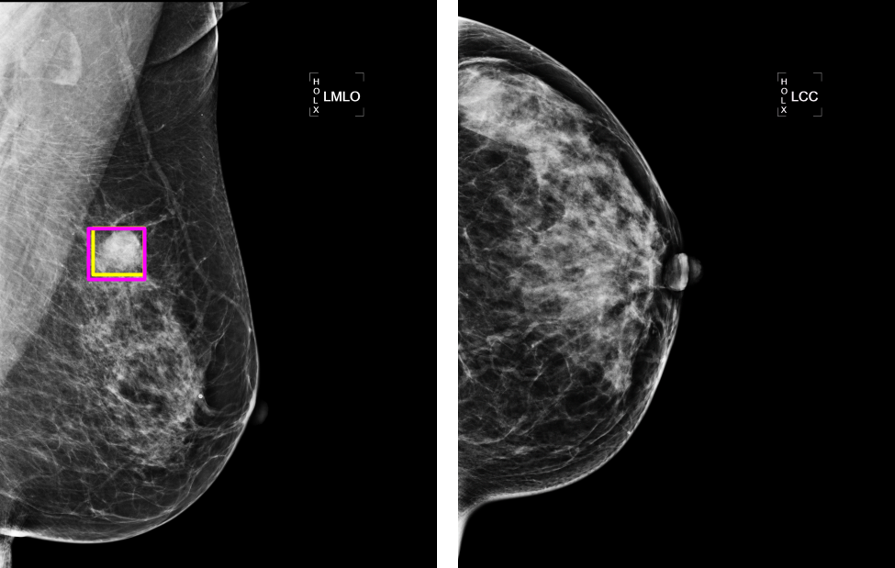
\includegraphics[width=0.40\textwidth]{stage2_pred_vis1}
    \bicaption{weakFaster R-CNN第二阶段对图片预测结果可视化}{Visualization of image prediction results in the second stage of a weakFaster R-CNN}
    \label{fig:stage2_pred_vis1}
\end{figure}

\section{本章小结}
本章对乳腺钼靶数据进行两阶段的考量和设计,第一阶段重点学习恶性样本中恶性病灶的信息,第二阶段着重学习区分正常样本中疑似恶性病灶和恶性病灶的区别,得到了基于weakFaster R-CNN训练下的乳腺钼靶数据预测结果。